\subsection*{Ход работы (измерение шумовых характеристик)}


\textbf{Шум осциллографа}.
Настроим осциллограф. Измерим параметры шума осциллографа. Для этого запустим построение гистограммы в режиме <<sample>> и получим из нее стандартное отклонение амплитуды шумов:
$$
\sigma_\text{osc} = 134.8\,\text{мкВ}.
$$

\textbf{Шум усилителя}.
Подключим в схему радиочастотный усилитель. Проведем для данной схемы измерения аналогичные предыдущему пункту:
$$
\sigma_\text{amp} = 1.195\,\text{мВ},
$$
при этом коэффициент усиления прибора равен: $G = 60$.

\textbf{Шум-факторы}.
Расчитаем шум-факторы входа осциллографа и усилителя:
$$
F = \frac{{S_\text{in}}/{N_\text{in}}}{{S_\text{out}}/{N_\text{out}}} = \frac{N_\text{out}}{GN_\text{in}}.
$$
Входной шум будем считать тепловым:
$$
N_\text{in} = \sqrt{4kTR\Delta f} = 1.42\cdot10^{-5}\,\text{В}.
$$
Тогда:
$$
F_\text{osc} = \frac{\sigma_\text{osc}}{N_\text{in}} = 9.5,
\hspace{5 mm} 
F_\text{amp} = \frac{\sigma_\text{amp}}{G\cdot N_\text{in}} = 1.4,
\hspace{10 mm} 
\frac{F_\text{amp}}{F_\text{osc}} = 0.15 < 1,
$$
а значит примем решение использовать усилитель, так как его шум-фактор ниже.

\textbf{Шум схемы}.
Подключим к получившемуся тракту источник-измеритель и измерительный модуль с фотодетектором. Убедимся, что напряжение на детектор подается в обратном смещении и произведем измерение шума полученной схемы при подаче напряжения в 0\,В.
$$
\sigma_\text{sys} = 1.259\,\text{мВ}.
$$


\textbf{Темновой ток}.
Произведем измерение темнового тока с учетом утечки:
$$
I_\text{full} = 5.24\pm 0.03\,\text{нА},\qquad I_\text{loss} = 0.010\pm 0.002\,\text{нА}
$$
Откуда темновой ток через фотодетектор равен:
$$
I_\text{dark} = I_\text{full} - I_\text{loss} = 5.23\pm 0.03\,\text{нА}.
$$


\begin{figure}[h]
    \centering
    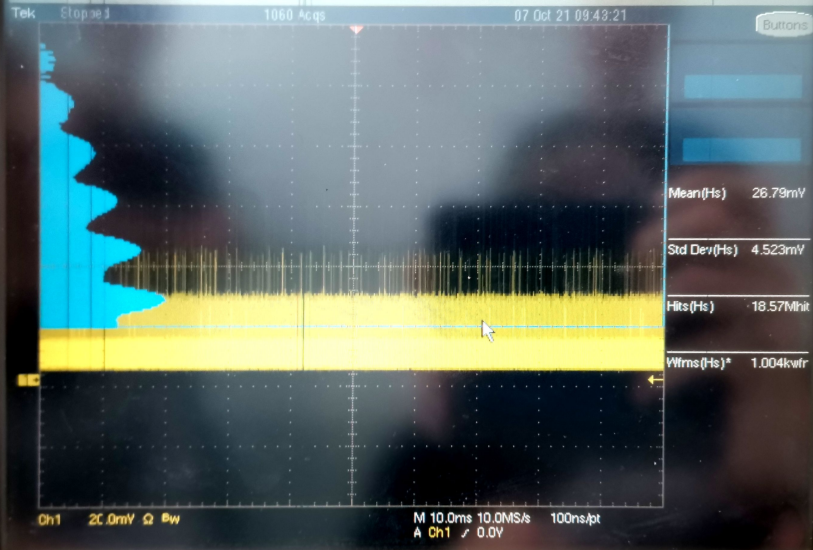
\includegraphics[width=0.45\textwidth]{figures/1.png}
    \hspace{5 mm} 
    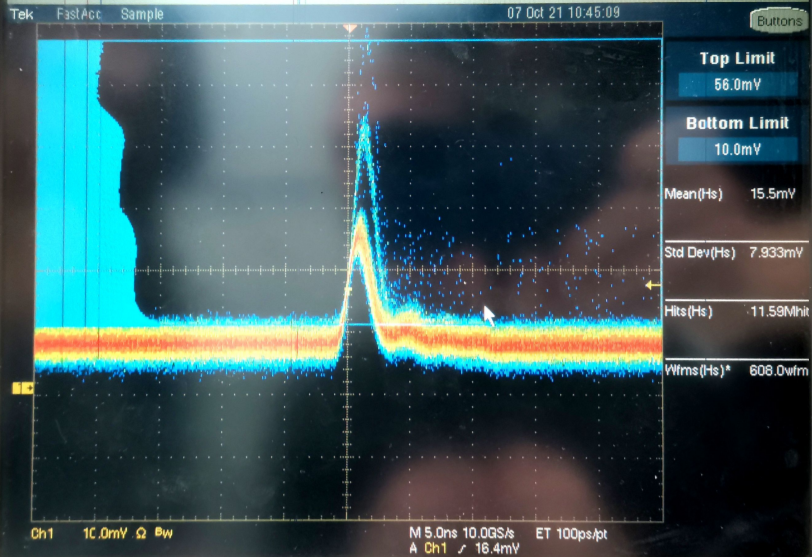
\includegraphics[width=0.45\textwidth]{figures/2.png}
    \caption{Осциллограммы детекции пиков и одиночных пиков.}
    \label{fig:0}
\end{figure}
